% *********************************************************************
% © 2021 Jeremy Sylvestre
%
% Permission is granted to copy, distribute and/or modify this document
% under the terms of the GNU Free Documentation License, Version 1.3 or
% any later version published by the Free Software Foundation; with no
% Invariant Sections, no Front-Cover Texts, and no Back-Cover Texts. A
% copy of the license is included in the appendix entitled “GNU Free
% Documentation License” that appears in the output document of this
% PreTeXt source code. All trademarks™ are the registered® marks of
% their respective owners.
%
% *********************************************************************

\newcommand*{\xmin}{-0.25}
\newcommand*{\xmax}{4}
\newcommand*{\ymin}{-2}
\newcommand*{\ymax}{2}

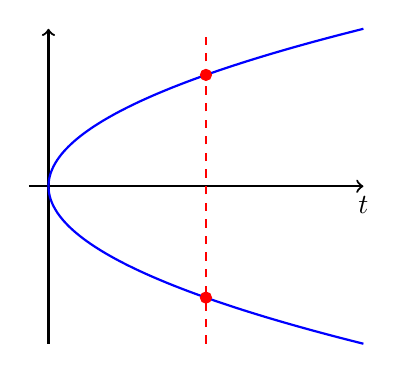
\begin{tikzpicture}
[
	closedpt/.style={circle,draw,fill,inner sep=0pt,minimum size=4pt},
	openpt/.style={circle,draw,inner sep=0pt,minimum size=4pt},
]

	% axes
	\draw[->,thick] (\xmin,0) -- (\xmax,0) node[below] {$t$};
	\draw[->,thick] (0,\ymin) -- (0,\ymax);

	% graph
	\draw[thick, blue, domain=0:2, smooth] plot ({\x * \x},\x);
	\draw[thick, blue, domain=0:2, smooth] plot ({\x * \x}, - \x);

	\draw[dashed,thick,red] (2,\ymin) -- (2,\ymax);
	\foreach \y in {1.414,-1.414}
		\node[red,closedpt] at (2,\y) {};

\end{tikzpicture}
